\subsection{Validation of TLP-HMM models and standard compliance}

\subsubsection{Model validation}

The response of the generator is tested in conditions as close as possible to the ISO 10605 standard \cite{iso10605}.
The generator is connected to a \SI{2}{\ohm} load, itself connected to a \SI{12}{\giga\hertz} (\SI{10}{\pico\second\per\sample}) oscilloscope with a \SI{50}{\ohm} input impedance.
The setup (Fig. \ref{fig:injection_setup_validation}) has the same loading impedance than the standard measurement "target" \cite{iso10605, iec61000-4-2}.

\begin{figure}[!h]
  \centering
  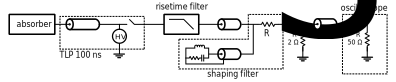
\includegraphics[width=0.9\textwidth]{src/5/figures/validation_injection_setup.pdf}
  \caption{Injection setup for validating the generator}
  \label{fig:injection_setup_validation}
\end{figure}

The measured and simulated waveforms are given in Fig. \ref{fig:tlp_hmm_waveforms}.
Measured currents at \SI{30}{\nano\second} and \SI{60}{\nano\second} are within the \SI{30}{\percent} tolerance of the standard (see Table \ref{tab:mes-sim-std-currents}).
The measured peak current is a bit lower (\SI{110}{\milli\ampere} short of minimum margin) than standard value.
This is easily corrected on the TLP by adding a small positive offset to the charging voltage.

\begin{figure}[!h]
  \centering
  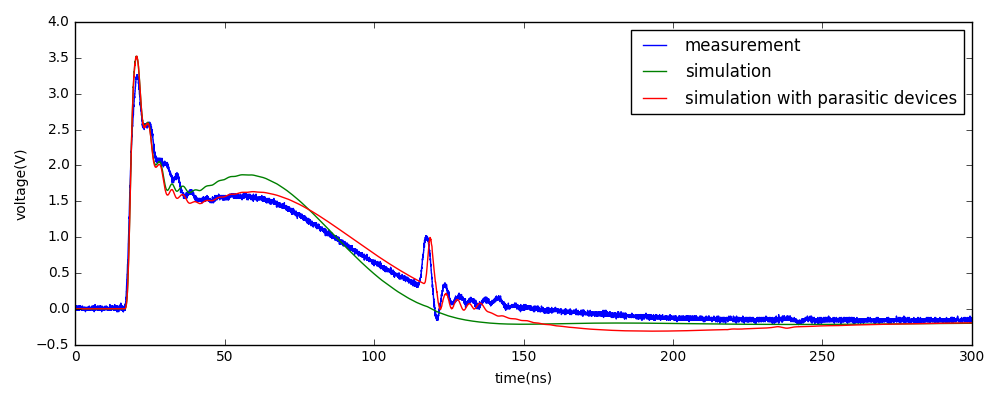
\includegraphics[width=0.95\textwidth]{src/5/figures/tlp_hmm_waveforms.png}
  \caption{Measurement versus simulation of a \SI{250}{\volt} TLP-HMM (equivalent \SI{1}{\kilo\volt} HMM) on \SI{2}{\ohm}}
  \label{fig:tlp_hmm_waveforms}
\end{figure}

\begin{table}[!h]
\centering
\begin{tabular}{@{}llll@{}}
\toprule
                            & Standard (A)    & Measured (A)  & Simulated (A) \\ \midrule
peak                        & 3.75 \pm 0.375  & 3.26          & 3.52 \\
\SI{30}{\nano\second}       & 2 \pm 0.6       & 1.54          & 1.8  \\
\SI{60}{\nano\second}       & 1 \pm 0.3       & 1.18          & 1.32 \\ \bottomrule
\end{tabular}
\caption{Measured and simulated currents versus standardized values}
\label{tab:mes-sim-std-currents}
\end{table}

% Analyse the curve
Overall, simulation and measurement correlate quite well.
There is a small difference for the slopes between \SI{40}{\nano\second} and \SI{150}{\nano\second}.
Investigation showed this difference comes from the shaping filter, and its inductances in particular.
Their frequency behavior is not as good as expected, and having four inductances in parallel increases further this issue.
Indeed, in this configuration parasitic capacitance of inductors are connected in parallel.
They add up together, leading to a large total parasitic value and degraded frequency behavior.
For the next iteration of the shaping filter, a single RF inductor should be used instead.
The shaping filter model can be corrected by connecting in parallel a total parasitic capacitance of \SI{2}{\nano\farad} in series with a \SI{15}{\ohm} parasitic resistor, like shown in Fig. \ref{fig:shaping_filter_schematic_parasitics}.

\begin{figure}[!h]
  \centering
  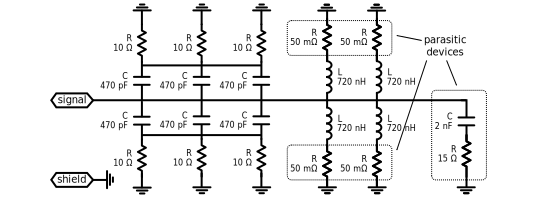
\includegraphics[width=0.8\textwidth]{src/5/figures/shaping_filter_schematic_parasitics.pdf}
  \caption{Shaping-filter schematic with parasitics}
  \label{fig:shaping_filter_schematic_parasitics}
\end{figure}

In Fig. \ref{fig:tlp_hmm_waveforms}, the glitch visible at approximately \SI{120}{\nano\second} is due to the absorber, because of two different parasitic devices.
At the beginning of the TLP pulse, the parasitic capacitance between signal and ground is charged.
Using the simulation, it is estimated at \SI{20}{\pico\farad}.
Its sudden discharge at the end of the TLP pulse causes the short voltage and current increase observed at \SI{120}{\nano\second}.
The parasitic series inductance of the three \SI{2.2}{\nano\farad} capacitors and the \SI{50}{\ohm} resistor (Fig. \ref{fig:absorber_schematic_parasitics}) is responsible afterward for the small oscillation observed between \SI{120}{\nano\second} and \SI{150}{\nano\second}.
This issue should be fixed in the next iteration of the absorber by building the absorber on a dedicated PCB with \SI{50}{\ohm} lines.
Guarantying matching along the path should eliminate this ringing oscillation.

\begin{figure}[!h]
  \centering
  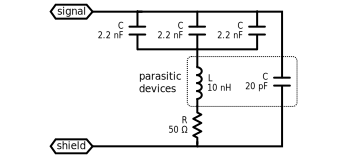
\includegraphics[width=0.5\textwidth]{src/5/figures/absorber_schematic_parasitics.pdf}
  \caption{Absorber schematic with parasitics}
  \label{fig:absorber_schematic_parasitics}
\end{figure}

\subsubsection{Comparison with an ESD Gun}

% Introduce how generators are usually tested against ESD gun
A generally adopted procedure to compare two ESD generators is to destroy ESD protections with each one of them and compare the failure levels.
Therefore, the TLP-HMM is compared to a real standardized HMM generator following this procedure.
The failure criteria is a sudden increase in the leakage current of the ESD protection under test after a pulse injection.

% Detail the devices that are going to be tested
A set of ten different ESD protections, of different size, on-resistance, structure and failure levels are stressed with both generators.
Five samples are tested for each structure and generator, to ensure the failure levels do not exhibit large variations.
Table \ref{tab:esd-protections} gives the on-resistance for each tested device.
These values are important later on for building a failure correlation method.

\begin{table}[!h]
\centering
\begin{tabular}{@{}lllllllllll@{}}
\toprule
Structure                          & A    & B    & C     & D    & E   & F   & G   & H   & I   & J   \\ \midrule
R\textsubscript{ON} (\textOmega{}) & 6.2  & 2.85 & 9.7  & 13.3 & 2.7 & 3.25& 2.4 & 4.7 & 1.7 & 1.85 \\
\end{tabular}
\caption{Tested ESD protection set}
\label{tab:esd-protections}
\end{table}

% Test results & limitations
Testing results are summarized in Table \ref{tab:esd-protections}.
Unfortunately, the result set is too small to draw a clear conclusion.
It was discovered that the TLP-HMM is not able to deliver enough current to break structure E and above.
The TLP-HMM relies on a regular TLP, whose high-voltage DC supply is limited to \SI{1}{\kilo\volt}.
On a true HMM generator, high-voltage \gls{dc} supplies are generally able to reach \SI{15}{\kilo\volt} charging voltage and beyond.
A TLP rarely requires DC supplies able to reach above \SI{1}{\kilo\volt}, because the output impedance is lower than HMM.
For a given charging voltage, a TLP will deliver a much larger amount of current than an HMM generator.
However, in the TLP-HMM configuration, the equivalent impedance of the generator is higher than the one of a TLP.
As a result, the injected current is smaller.
Ultimately, the TLP DC supply fails to charge high enough in order to produce large amounts of current.
This defect should be fixed in a new version by building a custom TLP with a much more powerful supply.

\begin{table}[!h]
\centering
\begin{tabular}{@{}lllllllllll@{}}
\toprule
Structure   & A     & B     & C      & D    & E    & F    & G     & H    & I     & J      \\ \midrule
TLP-HMM (V) & 640   & 700   & 890    & 860  & -    & -    & -     & -    & -     & -      \\
HMM     (V) & 1250  & 1250  & 1500   & 1500 & 6500 & 5000 & 13000 & 9500 & 20000 & 145000 \\
\end{tabular}
\caption{Testing results - failure levels per ESD protection}
\label{tab:esd-protections}
\end{table}

\subsubsection{Correlation between TLP and HMM}

% Correlation method principle orrelation results
Based on those preliminary results, a correlation method is built between TLP failure levels and HMM failure levels.
It exploits the fact that the TLP-HMM is at its core a TLP, yet has a similar behavior to an HMM generator.
The analysis was published in \cite{my-publi-tlp-hmm}.
It requires a very simple characterization step for each generator, to extract the most simple equivalent circuit composed of a resistor and a DC voltage source.
The DC voltage source takes the value defined by the user on the generator before a pulse.
The resistor is extracted from the characterization.
Finally, the ESD protection is modeled by its on-resistance.
The complete equivalent circuit is just a DC source with two resistors in series (Fig \ref{fig:simple_equivalent_circuit}).
The circuit is extremely simple, however it is shown later on that it is sufficient to build a seemingly good correlation method.
The key part of this approach is to consider the interaction between the on-resistance of the ESD protection and the equivalent resistance of the generator.

\begin{figure}[!h]
  \centering
  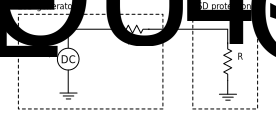
\includegraphics[width=0.65\textwidth]{src/5/figures/equivalent_circuit.pdf}
  \caption{Equivalent circuit for failure correlation}
  \label{fig:simple_equivalent_circuit}
\end{figure}

% What is equivalent resistance for each generator
Different equivalent DC voltages and resistances are found between TLP and HMM.
The TLP used in the NXP lab has an equivalent output resistance of \SI{83}{\ohm}.
Interestingly, a \SI{50}{\ohm} value was expected, but it turns out that this particular TLP has a mismatched attenuator in it, increasing slightly its equivalent output resistance.
A more classic TLP at the LAAS laboratory was also characterized and exhibits an output resistance of about \SI{53}{\ohm}.
The HMM generator has a much larger output resistance, estimated at about \SI{600}{\ohm}.
The TLP-HMM was also characterized, and situates somewhere in the middle with an output resistance of about \SI{300}{\ohm}.

\begin{figure}[!h]
  \centering
  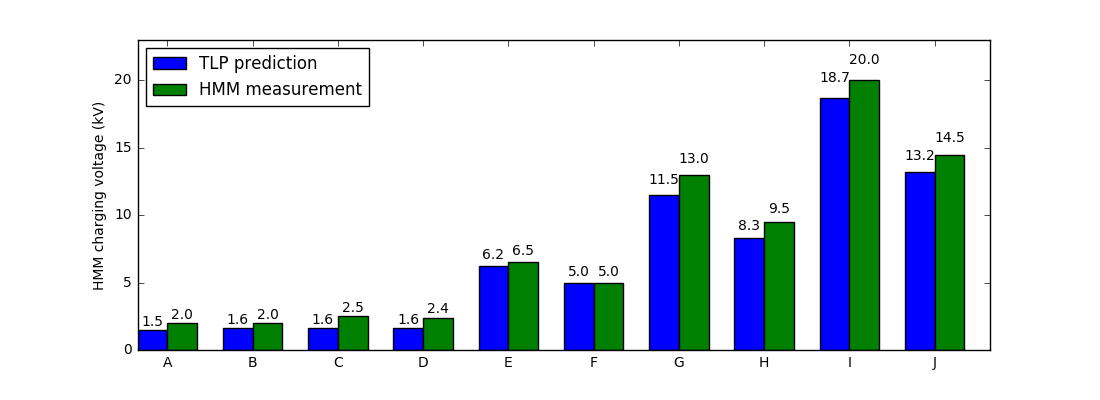
\includegraphics[width=0.95\textwidth]{src/5/figures/correlation_results.png}
  \caption{TLP prediction versus HMM measurement of failure levels}
  \label{fig:predicted_vs_measured_levels}
\end{figure}

% What is the discovered correlation
Despite different charging voltages and equivalent resistances, using this simple method yields almost identical failure currents between TLP and TLP-HMM.
I\textsubscript{ESD} (from Fig. \ref{fig:simple_equivalent_circuit}) was calculated with each generator, for each of the 10 tested structures.
This result indicates that this simplified circuit could link failure levels between generators.
To try this hypothesis further, it is attempted to predict the HMM failure levels, directly from TLP results.
The prediction method requires the TLP failure voltage and the ESD-on resistance, to predict the HMM failing voltage.
Both values are easily obtained from a TLP characterization.
Eq. \ref{eq:relation-prediction} provides the formula, directly extracted from the equivalent circuit, to link HMM charging voltage to the TLP failure current.
In this formula, I\textsubscript{ESD} is measured with the TLP.

\begin{equation}
V_{HMM} = I_{ESD} * (R_{HMM} + R_{ON})
\label{eq:relation-prediction}
\end{equation}

Fig. \ref{fig:predicted_vs_measured_levels} shows the results of this prediction method on the set of 10 ESD protections.
Good correlation is achieved and indicates this method could effectively be used to establish correlation between ESD generators.
